\chapter{贪心算法 (Greedy algorithms)}

像国际象棋这样的博弈游戏，只有深谋远虑、提前规划才能取胜：一个只顾眼前利益的棋手很容易被击败。然而在许多其他游戏（例如拼字游戏 Scrabble）中，人们只需简单地做出眼前看起来最好的一步，而不必过多担忧未来的连锁反应，就能取得相当不错的战绩。

这种“目光短浅”的行为简单而便捷，使其成为一种极具吸引力的算法设计策略。\textbf{贪心算法 (Greedy algorithms)} 通过一步一步构建解，在每一步中始终选择能够带来最明显、最直接即时效益的部分。尽管对于某些计算任务这种方法可能会导致灾难性的后果，但对于许多重要问题，贪心策略却是严格最优的。我们的第一个经典范例就是\textbf{最小生成树 (Minimum spanning trees)}。

\section{最小生成树 (Minimum spanning trees)}

假设你需要通过连接选定的计算机对，将一组计算机组网。这可以转化为一个图论问题：节点代表计算机，无向边代表潜在的通信链路，目标是挑选出足够多的边使得所有节点相互连通。但这还不是全部：每条链路都有维护成本，由该边的权重反映。怎样才是成本最低的可能网络？

\begin{figure}[htbp]
\centering
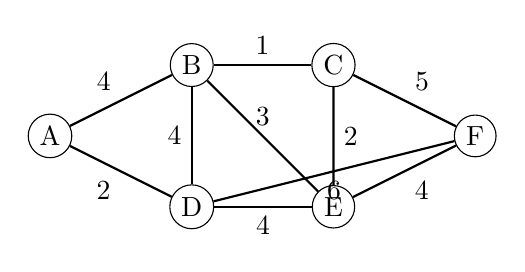
\begin{tikzpicture}[scale=0.9, auto, >=latex]
    \node[circle,draw,inner sep=2pt] (A) at (0,2) {A};
    \node[circle,draw,inner sep=2pt] (B) at (2,3) {B};
    \node[circle,draw,inner sep=2pt] (C) at (4,3) {C};
    \node[circle,draw,inner sep=2pt] (D) at (2,1) {D};
    \node[circle,draw,inner sep=2pt] (E) at (4,1) {E};
    \node[circle,draw,inner sep=2pt] (F) at (6,2) {F};

    \draw[thick] (A) -- node[above left] {4} (B);
    \draw[thick] (A) -- node[below left] {2} (D);
    \draw[thick] (B) -- node[above] {1} (C);
    \draw[thick] (B) -- node[left] {4} (D);
    \draw[thick] (B) -- node[above] {3} (E);
    \draw[thick] (C) -- node[above right] {5} (F);
    \draw[thick] (C) -- node[right] {2} (E);
    \draw[thick] (D) -- node[below] {4} (E);
    \draw[thick] (E) -- node[below right] {4} (F);
    \draw[thick] (D) -- node[below] {6} (F);
\end{tikzpicture}
\caption{计算机通信网络模型（边权代表维护成本）}
\label{fig:mst_network_intro}
\end{figure}

一个显而易见的观察是：最优的边集绝不能包含环路（回路），因为从环中移除任意一条边都会降低总成本，而绝不会破坏图的连通性：

\begin{property}
从图中的环路中移除任意一条边，不会破坏图的连通性。
\end{property}

因此，最优解必须既是连通的，又是不含环路的：这种无向图被称为\textbf{树 (tree)}。我们所寻求的特定树是总权重最小的生成树，被称为\textbf{最小生成树 (Minimum Spanning Tree，简称 MST)}。形式化定义如下：

\begin{tcolorbox}[colback=white,colframe=gray!50!black]
\textbf{最小生成树问题 (Minimum Spanning Tree)} \\
\textbf{输入：} 连通无向图 $G = (V, E)$；边权 $\{w_e : e \in E\}$ \\
\textbf{输出：} 生成树 $T = (V, E')$（其中 $E' \subseteq E$），使得总权重
\[
\text{weight}(T) = \sum_{e \in E'} w_e
\]
达到最小。
\end{tcolorbox}

在图 \ref{fig:mst_network_intro} 的例子中，最小生成树的成本为 16（包含边 $(B, C)$、$(A, D)$、$(C, E)$、$(A, B)$、$(E, F)$ 等）。

\begin{sidebarbox}{树的性质 (Trees)}
树是一个连通且无环的无向图。树之所以在计算机科学中如此有用，很大程度上源于其结构的纯粹与简明。例如：

\begin{property}
包含 $n$ 个节点的树恰好包含 $n - 1$ 条边。
\end{property}
这可以通过从空图开始一次添加一条边来构建树来证明：初始时 $n$ 个节点彼此孤立，各自属于独立的连通分量。每添加一条边，若该边连接两个不同的连通分量，则总连通分量数减少 1。最终形成单一连通分量时，必定恰好添加了 $n - 1$ 条边。

其逆命题同样成立：
\begin{property}
任何包含 $|V| - 1$ 条边的连通无向图 $G = (V, E)$ 必定是一棵树。
\end{property}

此外，树还具有路径唯一性特征：
\begin{property}
一个无向图是树，当且仅当图中任意两个节点之间存在\textbf{唯一}的一条简单路径。
\end{property}
\end{sidebarbox}

\subsection{贪心方法与 Kruskal 算法}

Kruskal 最小生成树算法从空图开始，依照如下简洁的规则从 $E$ 中挑选边：
\begin{center}
    \textbf{反复添加下一条权重最小且不会产生环路的边。}
\end{center}

换句话说，算法一条边一条边地构建树；除了小心避免形成环路之外，它在每一步仅仅贪心地挑选当前可用的最便宜的边。

\begin{figure}[htbp]
\centering
\begin{tcolorbox}[colback=white,colframe=gray!50!black,title={\textbf{图 5.4}\quad Kruskal 最小生成树算法}]
\begin{algorithmic}[1]
\Procedure{kruskal}{$G, w$}
    \State \textbf{Input:} 连通无向图 $G = (V, E)$，边权 $w_e$
    \State \textbf{Output:} 由边集 $X$ 定义的最小生成树
    \For{所有 $u \in V$}
        \State $\Call{makeset}{u}$
    \EndFor
    \State $X = \{\}$
    \State 将所有边 $E$ 按照权重非降序排序
    \For{每一条边 $\{u, v\} \in E$（按权重由小到大）}
        \If{$\Call{find}{u} \ne \Call{find}{v}$}
            \State 将边 $\{u, v\}$ 加入 $X$
            \State $\Call{union}{u, v}$
        \EndIf
    \EndFor
\EndProcedure
\end{algorithmic}
\end{tcolorbox}
\label{fig:kruskal_alg}
\end{figure}

\subsection{割性质 (The cut property)}

Kruskal 算法的正确性源于一条通用的\textbf{割性质 (Cut property)}，该性质足以证明一整批最小生成树算法的正确性。

\begin{lemma}[\textbf{割性质 (Cut property)}]
假设边子集 $X$ 是图 $G = (V, E)$ 某个最小生成树的一部分。选取任意一个节点子集 $S \subset V$，使得 $X$ 中没有任何边横跨在 $S$ 与 $V \setminus S$ 之间。令 $e$ 为横跨割 $(S, V \setminus S)$ 的所有边中权重最小的那条边。那么 $X \cup \{e\}$ 必然也是图 $G$ 某个最小生成树的一部分。
\end{lemma}

\begin{proof}
割（Cut）是指将顶点集划分为两部分 $S$ 与 $V \setminus S$。设 $X$ 属于某个最小生成树 $T$。若 $e \in T$，则结论显然成立。若 $e \notin T$，将 $e$ 加入 $T$ 必然产生一个环路。由于 $e$ 的端点分属 $S$ 与 $V \setminus S$，该环路上必然存在另一条横跨割 $(S, V \setminus S)$ 的边 $e'$。定义新生成树 $T' = T \cup \{e\} \setminus \{e'\}$。
由于 $e$ 是横跨该割的最小权边，必有 $w(e) \le w(e')$，因此：
\[
\text{weight}(T') = \text{weight}(T) + w(e) - w(e') \le \text{weight}(T).
\]
由 $T$ 的最小性可知 $\text{weight}(T') = \text{weight}(T)$，即 $T'$ 亦为最小生成树，且显然包含 $X \cup \{e\}$。
\end{proof}

\subsection{并查集数据结构 (A data structure for disjoint sets)}

为了高效执行 Kruskal 算法，需要一种数据结构来维护互不相交的集合：
\begin{itemize}
    \item \texttt{makeset(x)}：创建仅包含单个元素 $x$ 的集合；
    \item \texttt{find(x)}：返回 $x$ 所在集合的代表元；
    \item \texttt{union(x, y)}：合并包含 $x$ 与 $y$ 的两个集合。
\end{itemize}

\subsubsection*{按秩合并 (Union by rank)}
每个集合表示为一棵有向有根树。每个节点维护父指针 $\pi(x)$ 与秩 $\text{rank}(x)$（表示子树高度）。合并两个集合时，始终将秩较小的树的根指向秩较大的树的根；当两棵树的秩相同时，将其中一个指向另一个，并将新的根节点的秩加 1。

\begin{property}
使用按秩合并时，包含 $n$ 个元素的任意树的高度至多为 $\lfloor \log_2 n \rfloor$。因此单次 \texttt{find} 和 \texttt{union} 的时间复杂度均为 $O(\log n)$。
\end{property}

\subsubsection*{路径压缩 (Path compression)}
在执行 \texttt{find(x)} 时，顺着父指针向上查找到根节点后，直接将沿途访问过的所有节点的父指针全部重定向直连到根节点：
\begin{algorithmic}[1]
\Function{find}{$x$}
    \If{$x \ne \pi(x)$}
        \State $\pi(x) = \Call{find}{\pi(x)}$
    \EndIf
    \State \Return $\pi(x)$
\EndFunction
\end{algorithmic}

结合按秩合并与路径压缩后，一系列 $m$ 次操作的平均单次摊还时间降至 $O(\log^* n)$（阿克曼反函数 $\alpha(n)$ 级别），在所有实际应用中均小于等于 5，即近乎完美的常数时间 $O(1)$！

\subsection{Prim 算法 (Prim's algorithm)}

Prim 算法是最小生成树的另一种贪心策略：在算法执行的每一时刻，已挑选的边集 $X$ 始终构成一棵连通的子树，而 $S$ 恰好是该子树的顶点集。

在每次迭代中，树向外扩张一条边——即连接 $S$ 与 $V \setminus S$ 的最轻边。这与 Dijkstra 算法的结构惊人地相似，唯一的区别在于优先队列中的关键字定义：Dijkstra 关注的是从原点出发的整条路径长度，而 Prim 算法关注的是从集合 $S$ 连接到外界节点的单边权重 $\min_{u \in S} w(u, v)$。

\begin{figure}[htbp]
\centering
\begin{tcolorbox}[colback=white,colframe=gray!50!black,title={\textbf{图 5.9}\quad Prim 最小生成树算法}]
\begin{algorithmic}[1]
\Procedure{prim}{$G, w$}
    \State \textbf{Input:} 连通无向图 $G = (V, E)$，边权 $w_e$
    \State \textbf{Output:} 由前驱指针 $\text{prev}$ 定义的最小生成树
    \For{所有 $u \in V$}
        \State $\text{cost}(u) = \infty,\; \text{prev}(u) = \text{nil}$
    \EndFor
    \State 任意挑选起始节点 $u_0 \in V$，令 $\text{cost}(u_0) = 0$
    \State $H = \Call{makequeue}{V}$ \Comment{以 cost 值为关键字建立优先队列}
    \While{$H$ 非空}
        \State $v = \Call{deletemin}{H}$
        \For{每一条与 $v$ 相连的边 $\{v, z\} \in E$}
            \If{$z \in H$ \textbf{and} $\text{cost}(z) > w(v, z)$}
                \State $\text{cost}(z) = w(v, z)$
                \State $\text{prev}(z) = v$
                \State $\Call{decreasekey}{H, z}$
            \EndIf
        \EndFor
    \EndWhile
\EndProcedure
\end{algorithmic}
\end{tcolorbox}
\label{fig:prim_alg}
\end{figure}

\begin{sidebarbox}{用于最小割的随机化算法 (A randomized algorithm for minimum cut)}
生成树与割之间有着深厚的内在联系。考虑无向无权图 $G$，若我们在运行 Kruskal 算法时将所有边完全随机打乱顺序，并在生成树刚好剩下最后一条边未加入时（即图被缩减为恰好 2 个连通分量 $(S, V \setminus S)$）停机，该割 $(S, V \setminus S)$ 有至少 $1/\binom{n}{2} \ge 2/n^2$ 的概率恰好是图 $G$ 的\textbf{全局最小割 (Minimum Cut)}！

通过独立重复该过程 $O(n^2 \log n)$ 次并取最小值，我们便以极高概率找到了图的最小割。这是大卫·卡格尔（David Karger）提出的著名随机化收缩算法，也是目前求解最小割问题最快算法的基础。
\end{sidebarbox}

\section{Huffman 编码 (Huffman encoding)}

在 MP3 音频压缩等场景中，需要将长度为 $T$ 的字符序列转换为二进制存储。若字母表包含 4 个符号 $\{A, B, C, D\}$，朴素的固定长度编码每个符号需要 2 个比特（例如 $A: 00, B: 01, C: 10, D: 11$）。

但若各符号出现的频次极不均等（例如 $A$ 出现 7000 万次，而 $B$ 仅出现 300 万次），采用\textbf{变长编码 (Variable-length encoding)} 让高频字符使用较短的编码，能大幅节省空间。

为了确保解码的唯一性与无歧义性，编码必须满足\textbf{前缀无歧义性 (Prefix-free property)}：没有任何符号的编码是另一个符号编码的前缀。任何前缀码都可以自然地表示为一棵以各符号为叶节点的真二叉树（向左为 0，向右为 1）。

\begin{figure}[htbp]
\centering
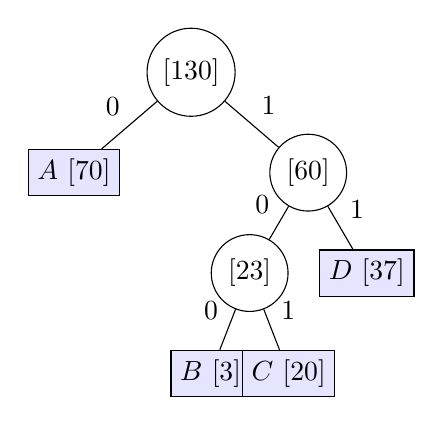
\begin{tikzpicture}[scale=0.85, level/.style={sibling distance=35mm/#1}]
    \node[circle,draw] {[130]}
        child {node[rectangle,draw,fill=blue!10] {$A$ [70]} edge from parent node[above left] {0}}
        child {node[circle,draw] {[60]}
            child {node[circle,draw] {[23]}
                child {node[rectangle,draw,fill=blue!10] {$B$ [3]} edge from parent node[above left] {0}}
                child {node[rectangle,draw,fill=blue!10] {$C$ [20]} edge from parent node[above right] {1}}
                edge from parent node[above left] {0}
            }
            child {node[rectangle,draw,fill=blue!10] {$D$ [37]} edge from parent node[above right] {1}}
            edge from parent node[above right] {1}
        };
\end{tikzpicture}
\caption{前缀编码树（方括号内为频数/权重）}
\label{fig:huffman_tree_demo}
\end{figure}

编码树的加权总代价为：
\[
\text{cost of tree} = \sum_{i=1}^n f_i \cdot (\text{符号 } i \text{ 的树深度}) = \sum_{\text{所有非根节点 } v} f(v).
\]

这启发了贪心构造方案：\textbf{每次找出当前频次最低的两个节点，将它们合并为一个新的父节点，其频次为两者之和，放入优先队列中重复此过程}。这就是经典的 \textbf{Huffman 算法}，耗时 $O(n \log n)$。

\begin{sidebarbox}{信息熵 (Entropy)}
概率分布的内在不可预测性或随机性可以通过压缩极限来量化。若 $n$ 个可能结果的出现概率分别为 $p_1, \dots, p_n$，则对单个事件编码所需的理论极限平均比特数由\textbf{香农熵 (Shannon entropy)} 给出：
\[
H(p) = \sum_{i=1}^n p_i \log_2 \frac{1}{p_i}.
\]
偏斜越严重的分布熵越低（更具可预测性，更容易被 Huffman 压缩）；均匀分布的熵最高。
\end{sidebarbox}

\section{Horn 公式 (Horn formulas)}

Horn 公式是逻辑推理与专家系统（如 Prolog 语言）中的核心知识表示形式。公式由两类子句构成：
\begin{enumerate}
    \item \textbf{蕴含式 (Implications)}：左侧为若干正文字的合取（AND），右侧为单个正文字。例如 $(z \land w) \implies u$。退化形式“$\implies x$”表示 $x$ 必然为真。
    \item \textbf{纯负子句 (Pure negative clauses)}：若干负文字的析取（OR），例如 $(\neg u \lor \neg v \lor \neg y)$，意即它们不能同时为真。
\end{enumerate}

目标是寻找一个使所有子句均成立的\textbf{真值满足赋值 (satisfying assignment)}。

\textbf{贪心（吝啬）策略}：
\begin{itemize}
    \item 初始时将所有布尔变量均置为 $\text{false}$；
    \item 只要存在某个蕴含式尚未被满足（即前提全为真而结论为假），就被迫且唯一地将右侧变量置为 $\text{true}$；
    \item 当所有蕴含式均被满足后，检查纯负子句是否全部成立：若成立则返回该赋值；若有冲突则断言该公式\textbf{不可满足}。
\end{itemize}
该贪心算法可在关于公式长度线性的时间 $O(L)$ 内执行完毕。

\section{集合覆盖 (Set cover)}

\begin{tcolorbox}[colback=white,colframe=gray!50!black]
\textbf{集合覆盖问题 (Set Cover)} \\
\textbf{输入：} 基础元素集合 $B$；子集族 $S_1, \dots, S_m \subseteq B$ \\
\textbf{输出：} 一个选取的子集族集合，其并集覆盖 $B$，且选取的集合数量尽量少。
\end{tcolorbox}

\textbf{贪心策略}：重复执行直到所有元素被覆盖——每次挑选能够覆盖最多未覆盖元素的子集 $S_i$。

\begin{claim}
若基础集合包含 $n$ 个元素，且最优覆盖由 $k$ 个集合组成，则贪心算法选取的集合数量至多为 $k \ln n$。
\end{claim}

\begin{proof}
设经过 $t$ 轮后剩余未覆盖元素个数为 $n_t$（$n_0 = n$）。因为最优解用 $k$ 个集合就能覆盖这 $n_t$ 个元素，根据鸽巢原理，必定存在某个子集至少能覆盖其中的 $n_t / k$ 个元素。因此贪心选择保证：
\[
n_{t+1} \le n_t - \frac{n_t}{k} = n_t \left(1 - \frac{1}{k}\right) \le n_0 \left(1 - \frac{1}{k}\right)^{t+1} < n e^{-(t+1)/k}.
\]
当 $t = k \ln n$ 时，未覆盖元素数 $n_t < n e^{-\ln n} = 1$，意味着所有元素已被全部覆盖。
\end{proof}
因此贪心算法的近似比（Approximation factor）为 $\ln n$。

\newpage
\section*{习题 (Exercises)}
\addcontentsline{toc}{section}{习题}

\begin{exercise}{5.1}
计算给定图的最小生成树成本与数量，并给出 Kruskal 算法添加边的顺序及每次对应的割。
\end{exercise}

\begin{exercise}{5.2}
在给定图上分别模拟 Prim 算法与带路径压缩的 Kruskal 算法。
\end{exercise}

\begin{exercise}{5.3}
设计线性时间 $O(|V|)$ 算法，判断连通无向图中是否存在一条可删除且不破坏连通性的边。
\end{exercise}

\begin{exercise}{5.4}
证明包含 $n$ 个顶点和 $k$ 个连通分量的无向图至少包含 $n - k$ 条边。
\end{exercise}

\begin{exercise}{5.5}
边权同时增加 1 时，分析最小生成树与单源最短路径是否会发生改变。
\end{exercise}

\begin{exercise}{5.6}
证明若无向图中所有边权两两互异，则最小生成树唯一。
\end{exercise}

\begin{exercise}{5.7}
给出寻找图的最大生成树（总权重最大的生成树）的算法。
\end{exercise}

\begin{exercise}{5.8}
探讨最短路径树与最小生成树是否可能完全不共享任何公共边。
\end{exercise}

\begin{exercise}{5.9}
最小生成树的 10 个经典性质正误判断与证明/反例。
\end{exercise}

\begin{exercise}{5.10}
设 $T$ 为 $G$ 的 MST，$H$ 为连通子图，证明 $T \cap H$ 包含在 $H$ 的某个 MST 中。
\end{exercise}

\begin{exercise}{5.11}
跟踪带路径压缩的并查集在给定操作序列下的树形态。
\end{exercise}

\begin{exercise}{5.12}
证明仅使用按秩合并而不进行路径压缩时，存在最坏情况耗时 $\Omega(m \log n)$ 的操作序列。
\end{exercise}

\begin{exercise}{5.13}
根据给定 DNA 碱基频率（A: 31\%, C: 20\%, G: 9\%, T: 40\%）构造最优 Huffman 编码。
\end{exercise}

\begin{exercise}{5.14}
计算给定 5 个字符频率下的 Huffman 树及其对 100 万字符文件的压缩比特数。
\end{exercise}

\begin{exercise}{5.15}
探讨给定前缀码是否可能由 Huffman 算法生成。
\end{exercise}

\begin{exercise}{5.16}
证明 Huffman 编码的长度特征：(a) 若某字符频率 $> 2/5$，则必存在长度为 1 的编码；(b) 若所有字符频率 $< 1/3$，则绝不存在长度为 1 的编码。
\end{exercise}

\begin{exercise}{5.17}
分析 $n$ 个符号的 Huffman 编码中可能出现的最长编码长度及对应频率构造。
\end{exercise}

\begin{exercise}{5.18}
英语字母统计频率的 Huffman 最优编码与香农熵对比。
\end{exercise}

\begin{exercise}{5.19}
信息熵极值分析：证明均匀分布时熵最大，退化分布时熵最小。
\end{exercise}

\begin{exercise}{5.20}
设计线性时间算法判断树结构是否存在完美匹配（Perfect matching）。
\end{exercise}

\begin{exercise}{5.21}
利用最大生成树求解无向图的最小权反馈边集（Feedback edge set）。
\end{exercise}

\begin{exercise}{5.22}
逆向删除法求 MST：每次删除当前最重且位于环上的边。
\end{exercise}

\begin{exercise}{5.23}
单条边权重更新时，在线性时间 $O(|V|)$ 内动态维护最小生成树。
\end{exercise}

\begin{exercise}{5.24}
求解指定子集 $U$ 的所有节点必须全部作为叶节点的最轻生成树。
\end{exercise}

\begin{exercise}{5.25}
二进制计数器的自增与重置操作的 $O(1)$ 摊还复杂度证明。
\end{exercise}

\begin{exercise}{5.26}
程序变量等式与不等式约束系统的并查集判定算法。
\end{exercise}

\begin{exercise}{5.27}
度序列的可图化判定（Havel-Hakimi 定理的贪心算法）。
\end{exercise}

\begin{exercise}{5.28}
派对邀请名单优化问题（度数双重约束）。
\end{exercise}

\begin{exercise}{5.29}
证明极小前缀无歧义编码必对应一棵真二叉树。
\end{exercise}

\begin{exercise}{5.30}
三进制（Ternary）存储介质下的 Huffman 算法设计与正确性证明。
\end{exercise}

\begin{exercise}{5.31}
非等代价编码模型下的最优前缀码设计。
\end{exercise}

\begin{exercise}{5.32}
多客户排队等待时间最小化（SJF 贪心调度）。
\end{exercise}

\begin{exercise}{5.33}
Horn 公式可满足性贪心算法的线性时间实现。
\end{exercise}

\begin{exercise}{5.34}
构造集合覆盖实例，证明贪心算法的 $\ln n$ 近似界是紧确的（Tight）。
\end{exercise}

\begin{exercise}{5.35}
证明包含 $n$ 个节点的无向无权图最多包含 $\binom{n}{2}$ 个不同的全局最小割。
\end{exercise}
